\documentclass[conference]{IEEEtran}
\IEEEoverridecommandlockouts
% The preceding line is only needed to identify funding in the first footnote. If that is unneeded, please comment it out.
\usepackage{cite}
\usepackage{amsmath,amssymb,amsfonts}
\usepackage{algorithmic}
\usepackage{graphicx}
\usepackage{textcomp}
\usepackage{multirow}
\usepackage{pifont}
\usepackage{xcolor}
\usepackage{comment}
\usepackage{float} % 在导言区加

\def\BibTeX{{\rm B\kern-.05em{\sc i\kern-.025em b}\kern-.08em
    T\kern-.1667em\lower.7ex\hbox{E}\kern-.125emX}}

\begin{document}

\title{SAF-Mamba: Scale-Aware Mamba with Adaptive Frequency Filters for Cardiac Image Segmentation}

\author{\IEEEauthorblockN{
		Xinyi Luo, Shaoyu Wang\IEEEauthorrefmark{1},
		Nuo Chen, Shiying Yang,
		Xiujin Shi}
\IEEEauthorblockA{\textit{School of Information and Intelligence Science, Donghua University, Shanghai, China}\\
\IEEEauthorrefmark{1}Corresponding author, Email: sywang@dhu.edu.cn}}



\maketitle

\bstctlcite{IEEEexample:BSTcontrol}


\begin{abstract}
Cardiac image segmentation is essential for detecting and treating cardiovascular diseases. Scale variation and boundary displacement remain key challenges affecting segmentation accuracy. Existing CNN-based and ViT-based methods struggle to address these issues. Inspired by Mamba, a state space model capable of modeling both global and local context, we propose SAF-Mamba, a Mamba-based cardiac segmentation model with scale-aware and adaptive filtering. Specifically, SAF-Mamba employs a multi-scale Visual State Space (MSVSS) block to capture scale-dependent variations in cardiac images, where multi-scale depth-wise convolutions and the VSS block provide complementary context for comprehensive pattern recognition. Furthermore, adaptive filter blocks (AFBs) preserve fine details, with filters generated by an adaptive filter generator (AF Generator) that dynamically modulates frequency components to enhance boundary sharpness. Experiments on the ACDC and M\&Ms datasets yield Dice Similarity Coefficients of 92.21\% and 88.43\%, respectively, surpassing CNN-based, Transformer-based, and Mamba-based methods and demonstrating accurate and robust cardiac segmentation.
\end{abstract}

\begin{IEEEkeywords}
Cardiac image segmentation, Mamba, state space model, frequency domain analysis
\end{IEEEkeywords}

\section{Introduction}

Cardiovascular diseases (CVDs) are the leading cause of death globally \cite{WHO}, making accurate diagnosis and treatment planning essential. Automatic segmentation of cardiac magnetic resonance (CMR) images enables efficient assessment of cardiac morphology and supports clinical diagnosis, treatment, and prognosis.

Deep learning has become the dominant approach for medical image segmentation. CNN-based models like U-Net\cite{ronnebergerUNetConvolutionalNetworks2015} provide strong baselines but have limited receptive fields, while Transformer-based methods, such as Swin-Unet\cite{SwinUnetUnetlikePure2021a} and ViTs\cite{dosovitskiyImageWorth16x162021}, incur high computational cost on high-resolution cardiac images. Recently, Mamba\cite{MambaLinearTimeSequence2023}, derived from state space models (SSMs)\cite{EfficientlyModelingLong2022}, has shown promise by combining long-range dependency modeling with linear complexity. VMamba\cite{VMambaVisualState2024} extends Mamba to vision via the Visual State Space (VSS) block, mitigating direction-sensitivity between 1D sequences and 2D images. However, existing Mamba-based methods still struggle with challenges specific to cardiac segmentation, such as varying substructure scales and precise boundary delineation.

To address these issues, we propose SAF-Mamba, a scale-aware Mamba with adaptive frequency filters. We design the multi-scale Visual State Space (MSVSS) block, comprising parallel multi-scale depth-wise convolutions, a channel integration branch, and a calibration branch, to better capture scale variations. To preserve fine-grained features in the encoder, we introduce the Adaptive Filter Block (AFB) in skip connections, which enhances frequency components of multi-stage features. The filters adapt dynamically as high-, low-, or band-pass based on input features. In summary, the main contributions of this work are as follows:


\begin{figure*}[t]
\centering
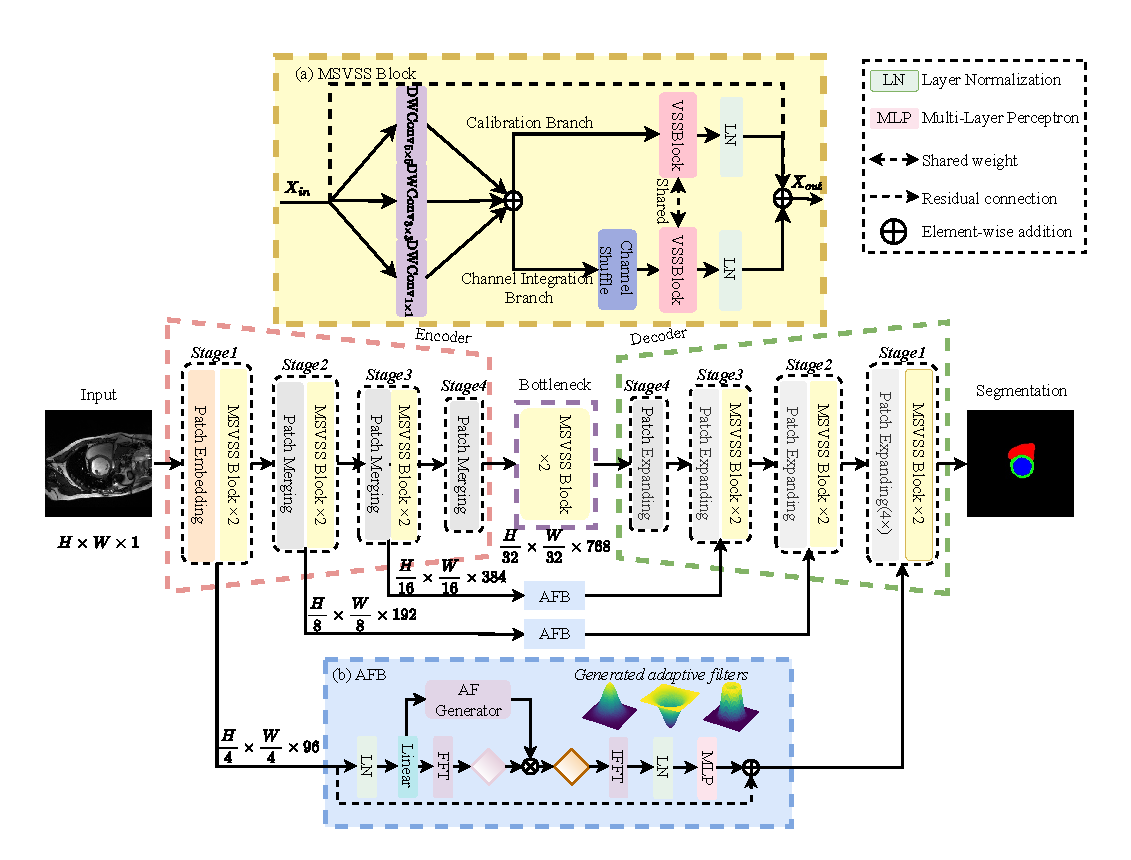
\includegraphics[width=\textwidth]{model_new.pdf}
\caption{\fontsize{8}{10}\selectfont {Overview of SAF-Mamba}. (a)  An illustration of multi-scale Visual State Space (MSVSS) Block. (b) The illustration of the apative filter block (AFB).}
\label{model}
\end{figure*}

\begin{itemize}
    \item We propose SAF-Mamba, a scale-aware Mamba with multi-scale Visual State Space (MSVSS) blocks and Adaptive Filter Blocks (AFB).  
    \item Experimental results show that SAF-Mamba enhances sensitivity to scale variations and boundary delineation on two challenging cardiac image datasets.
\end{itemize}




\begin{comment}
    \section{Related Work}
\subsection{State Space Models}
Recently, State Space Models have become a trending topic due to its ability to model long-range dependencies while maintaining linear complexity with respect to  the input sequence length.
Mamba has been successfully extended to vision tasks, with Vision Mamba\cite{VisionMambaEfficient2024} pioneering its application to 2D image data and Mamba-UNet\cite{MambaUNetUNetPureVisual2024} further enhancing medical image segmentation by integrating Mamba’s global context modeling into a U-Net framework. Other methods  have also demonstrated the effectiveness of Mamba in medical image segmentation. Inspired by Mamba-UNet, our MSVSS block enhances the VSS block by incorporating multi-scale depth-wise convolutions, allowing  SAF-Mamba to better adapt to scale variations in cardiac anatomical structures.

\subsection{Frequency Domain Learning}
%The discrete cosine transform (DCT) is incorporated in \cite{FcaNetFrequencyChannel2021} to replace the traditional global average pooling, which generalizes the existing channel attention mechanism in the frequency domain.
The Fourier Transform (FT) is a fundamental technique in frequency domain analysis and has been applied  across various computer vision tasks in recent years. Early methods primarily focused  on  feature extraction in the frequency domain, using FT to convert between spatial and frequency domains. For example, DFFormer\cite{FFTbasedDynamicToken2023} utilizes the dynamic weighted filters as the token mixer.
%to learn long-term spatial dependencies in the frequency domain, rather than the self-attention layer in vision transformers. 
Some studies have incorporated FT into medical image segmentation. EM-Net\cite{EMnetEfficientChannel2024} applies learnable weight parameters to frequency features for efficient frequency domain learning. Our AFB is closely related to frequency filtering methods. Unlike previous approaches that specify a fixed filter type, our filters in AFB can dynamically transform into high-pass, low-pass or band-pass based on the input features, those to be filtered. This flexibility allows the preservation of high-frequency boundary detail while maintaining low-frequency semantic features. 
%to preserve high-frequency edge features in the early encoder layers and incorporates low-frequency semantic features from the high-level features.
\end{comment}



\section{Method}

\subsection{Overview Architecture}
As shown in Fig.~\ref{model}, our proposed SAF-Mamba adopts a U-shaped hierarchical structure with skip connections. The encoder has four stages, beginning with patch embedding, which divides the input $I \in \mathbb{R}^{H \times W \times 1}$ into $\frac{H}{4} \times \frac{W}{4}$ non-overlapping patches and linearly projects them to 96 dimensions. These tokens pass through multiple MSVSS blocks for feature extraction, followed by patch merging layers that halve spatial dimensions and double channel depth, forming hierarchical representations. In the decoder, feature maps are upscaled via patch expanding and concatenated with outputs from corresponding AFBs in the first three encoder stages. Finally, patch expanding performs $4\times$ upsampling to produce a segmentation mask matching the input size.


\subsection{Multi-Scale VSS Block}
A persistent challenge in cardiac image segmentation lies in adapting to scale variations. Inspired by the fact that different convolution kernel sizes yield diverse receptive fields \cite{10006743}, we propose the MSVSS block, including parallel multi-scale depth-wise convolutions, a channel integration branch, and a calibration branch. Specifically, parallel depth-wise convolutions\cite{EMCADEfficientMultiscale2024} extract multi-scale features, while the integration branch uses channel shuffle\cite{ShuffleNetExtremelyEfficient2017} to capture inter-channel dependencies. The calibration branch refines features overlooked during integration. To achieve both global context and local scale awareness, the two branches share a VSS block built on scale-aware feature maps, ensuring comprehensive representation with reduced complexity. As shown in Fig.~\ref{model}(a), multi-scale features are derived from the input $\textbf{X}_{in} \in \mathbb{R}^{H \times {W} \times {C}}$ as:
\begin{equation}
\textbf{Y} =\text{DWConv}_{ks}(\textbf{X}_{in}),
\end{equation}
where $\text{DWConv}_{ks}(\cdot)$ denotes a depth-wise convolution with kernel size $ks$, and $\text{KS}={1\times1, 3\times3, 5\times5}$.

\begin{comment}
The VSS block used in our two branches is an visual extension of the Mamba block, which originates from State Space Models (SSMs), which represent continuous systems. For a system with input $x (t)$, the output $ y (t) $ can be obtained though a latent space representation $ h(t)$ as described in \eqref{Eq} :
\begin{equation}
\begin{aligned} 
h'(t) &= \mathbf{A}h(t) + \mathbf{B}x(t) \\
y(t) &= \mathbf{C}h(t) + \mathbf{D}x(t) 
\end{aligned} 
\label{Eq}
\end{equation}
where $\mathbf{A} $, $\mathbf{B} $, $\mathbf{C} $, and $\mathbf{D} $ are learnable parameters.
\end{comment}

The multi-scale features are then fed into the channel integration and calibration branch to capture inter-channel dependencies and refine the extracted features, as described in the following equations: 
\begin{equation}
\begin{aligned} 
\textbf{Y}_{1}&=\text{VSS}_{\text{shared}}(\text{Channel\:Shuffle}(\textbf{Y}))\\
\textbf{Y}_{2} &=\text{VSS}_\text{shared}(\textbf{Y})
\end{aligned} 
\end{equation}
Finally, the output $\textbf{X}_{out} \in \mathbb{R}^{H \times {W} \times {C}}$ can be obtained through the sum of $\textbf{Y}_{1}$ , $\textbf{Y}_{2}$  and residual connection from  $\textbf{X}_{in}$.

\begin{comment}
    \subsection{Adaptive Filter Block}
Another issue affecting cardiac image segmentation is that the successive downsampling operations in hierarchical encoder may cause the loss of important spatial features (e.g., edges, shapes) in the shallow stages and semantic features in the deeper stages. 
    Recent studies \cite{FEVADHighlowFrequency2024} indicate that high-frequency features are sensitive to capturing finer details, whereas low-frequency features correspond better to high-level semantics. On the basis of this, 
We propose the Adaptive Filtering Block (AFB), which applies adaptive filtering to the encoder features within the skip connections. As shown in Fig.~\ref{model}(b),  the spatial representation  $\textbf{X}_{i}\in \mathbb{R}^{H \times {W} \times {C}}$  is first processed through layer normalization (LN) and then projected into $\mathbf{\hat{X}}_{i}\in \mathbb{R}^{H \times {W} \times {2C}}$ using a linear layer. This is followed by a transformation into the spectral space. As many previous studies demonstrated\cite{FFTbasedDynamicToken2023}\cite{EMnetEfficientChannel2024}, the 2D discrete Fourier transform (DFT) is widely used to map a discrete finite signal into frequency components, which is defined as:
\begin{equation}
F(u, v) = \sum_{h=0}^{H-1} \sum_{w=0}^{W-1} f(h, w) \cdot e^{-j 2 \pi \left( \frac{ h u}{H} + \frac{w v}{W} \right)}
\end{equation}
where j is the imaginary unit, $f(h,w)$ represents the intensity value at position $(h, w)$ of the image in spatial domain and $F(u,v)$ denotes the complex frequency values, with $(u,v)$ representing  the coordinates of a spectrum in  frequency domain. 

To efficiently compute the 2D DFT, we employ the 2D fast Fourier transform (FFT) to convert features into the frequency domain. Adaptive filters generated by the adaptive filter generator (AF Generator) then enhance relevant frequency components while suppressing noise. The inverse FFT (IFFT) reconstructs refined features in the spatial domain. The above process can be depicted as:
\begin{equation}
A(\mathbf{\hat{X}}_i)=\mathcal{F}^{-1}(\mathcal{F}(\mathbf{\hat{X}}_{i}) \odot \textbf{F}_{c})
\end{equation}
where $\odot$ denotes the element-wise product,  $\mathcal{F}(\cdot)$ represents  2D FFT and $\mathcal{F}^{-1}(\cdot)$ is 2D IFFT. $\textbf{F}_{c}$ , generated by AF Generator, modulates the spectrum by emphasizing or suppressing specific frequency components based on input characteristics. A multi-layer perceptron (MLP) further models cross-channel dependencies and refines representations. The final output $\mathbf{X}^{out}_{i}\in \mathbb{R}^{H \times W \times C}$ is obtained by fusing with the residual input, recovering spatial details.
    modulates the feature's spectrum,  enhancing high-frequency components while suppressing low-frequency  ones (or vice versa), which depends on the  characteristics of  $\textbf{F}_{c}$  learned from the input. Subsequently, a multi-layer perceptron (MLP) layer is used to model cross-channel dependencies and further refine the feature representation. Finally, the refined output feature $\mathbf{X}^{out}_{i}\in \mathbb{R}^{H \times {W} \times {C}}$ is obtained by  fusing it with the residual input, enabling the recovery of spatial details and ensuring robust feature integration across scales. 
% which facilitates 

\begin{figure}[htbp]
\centering
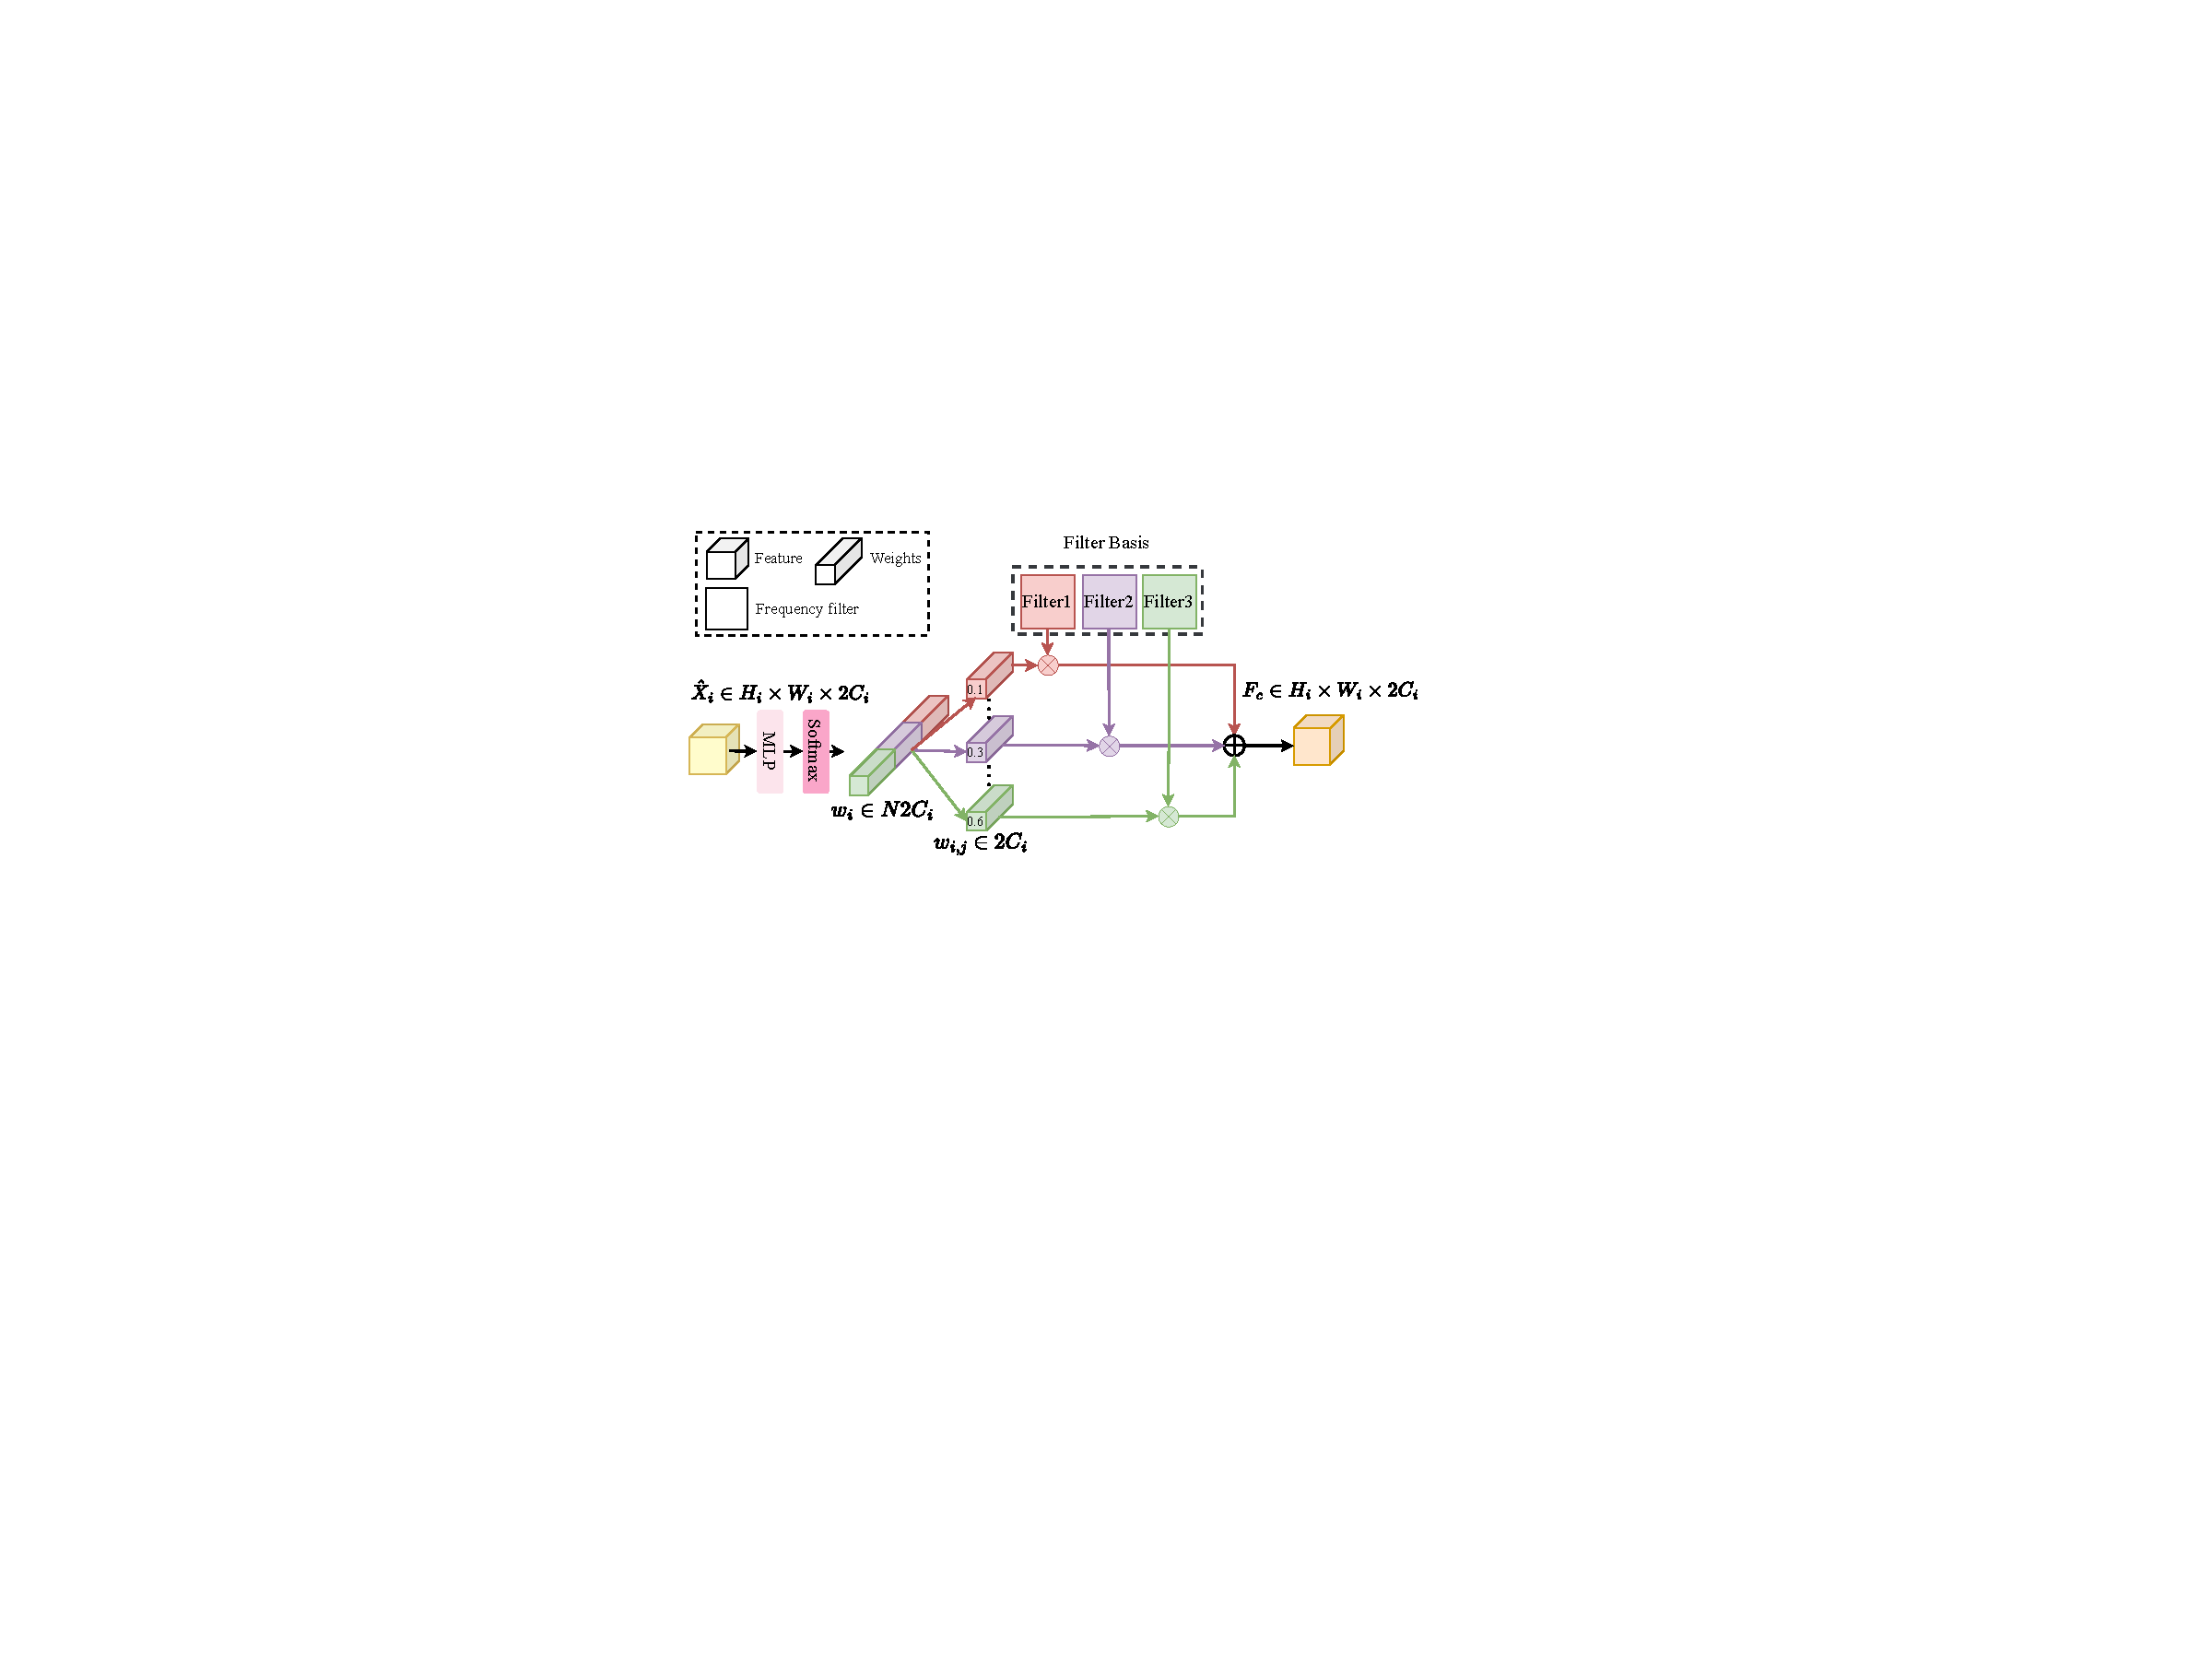
\includegraphics[width=\columnwidth]{AFG.pdf}
\caption{\fontsize{8}{10}\selectfont An illustration of the Adaptive Filter Generator (AF Generator). }
\label{afg}
\end{figure}

\textbf{Adaptive Filter Generator:}
%用MLP生成weight 进行加权求和得到filter
To generate adaptive filters, an MLP layer followed by softmax normalization produces channel-wise weights that linearly combine a filter basis $\mathbb{M}={\mathcal{M}1,\ldots,\mathcal{M}N}$, where each $\mathcal{M}i\in\mathbb{C}^{H\times\lceil\frac W2\rceil}$ is a randomly initialized complex parameter. As each spectral channel represents distinct frequency responses, channel-wise filtering is applied in the AFB, as shown in Fig.~\ref{afg}.
The weights are computed as: 
\begin{equation}
\mathbf{a}=\text{Softmax}\left(\text{MLP}\left(\frac{\sum_{h=1}^{\text{H}}\sum_{w=1}^{\text{W}} \mathbf{X}_{:,h,w}}{{\text{H}}{\text{W}}}\right)\right)
\end{equation}
\begin{equation}\mathbf{a}=(\alpha_1,\ldots,\alpha_{N2C})^{\top}
\end{equation}
where $\mathbf{a}\in \mathbb{R}^{N2C}$ is a vector for weighting filter basis to generate adaptive filters. Finally, the adaptive filters $\mathbf{F}_{c} \in\mathbb{C}^{ H\times\lceil\frac W2\rceil\times2C}$  are computed by the following equation: 
\begin{equation}
    \mathbf{F}_c = \sum_{i=1}^{N} \left( \frac{e^{\alpha_{c,i}}}{\sum_{n=1}^{N} e^{\alpha_{c,n}}} \right) \mathcal{M}_i
\end{equation}
where $\alpha_{c,i}$ denotes the $i$-th element of $\alpha$ for the $c$-th group. The vector $\alpha$ is divided into $N$ segments of length $2C$. In our model, $N=3$, matching the dimension of $\mathbb{M}$. Larger $N$ increases computational cost, while smaller values (e.g., $N=1$) make the adaptive filters degenerate into fixed ones.
\end{comment}

\subsection{Adaptive Filter Block}
Another issue affecting cardiac image segmentation is that the successive downsampling operations in hierarchical encoder may cause the loss of important spatial features (e.g., edges, shapes) in the shallow stages and semantic features in the deeper stages. We propose the Adaptive Filtering Block (AFB), which performs adaptive frequency filtering on encoder features via skip connections. As shown in Fig.~\ref{model}(b), the spatial feature $\textbf{X}{i}\in \mathbb{R}^{H \times W \times C}$ is normalized (LN), projected to $\mathbf{\hat{X}}{i}\in \mathbb{R}^{H \times W \times 2C}$ through a linear layer, and then transformed into the spectral domain. Following prior works\cite{FFTbasedDynamicToken2023,EMnetEfficientChannel2024}, we use the 2D discrete Fourier transform (DFT) to decompose spatial signals into frequency components.
\begin{comment}
    :
\begin{equation}
F(u, v) = \sum_{h=0}^{H-1} \sum_{w=0}^{W-1} f(h, w) \cdot e^{-j 2 \pi \left( \frac{ h u}{H} + \frac{w v}{W} \right)},
\end{equation}
where $j$ is the imaginary unit, $f(h,w)$ is the spatial intensity at $(h,w)$, and $F(u,v)$ denotes complex frequency values.
\end{comment}

To accelerate computation, the 2D fast Fourier transform (FFT) is used to map features into the frequency domain. Adaptive filters generated by the AF Generator enhance informative frequencies and suppress noise, after which the inverse FFT (IFFT) reconstructs refined spatial features:
\begin{equation}
A(\mathbf{\hat{X}}i)=\mathcal{F}^{-1}(\mathcal{F}(\mathbf{\hat{X}}{i}) \odot \textbf{F}_{c}),
\end{equation}
where $\odot$ denotes element-wise multiplication, $\mathcal{F}(\cdot)$ and $\mathcal{F}^{-1}(\cdot)$ represent 2D FFT/IFFT, and $\textbf{F}{c}$ modulates the spectrum based on input characteristics. A multi-layer perceptron (MLP) further models cross-channel dependencies and refines features. The final output $\mathbf{X}^{out}_{i}\in \mathbb{R}^{H \times W \times C}$ is obtained by residual fusion, recovering spatial details.

\begin{figure}[htbp]
\centering
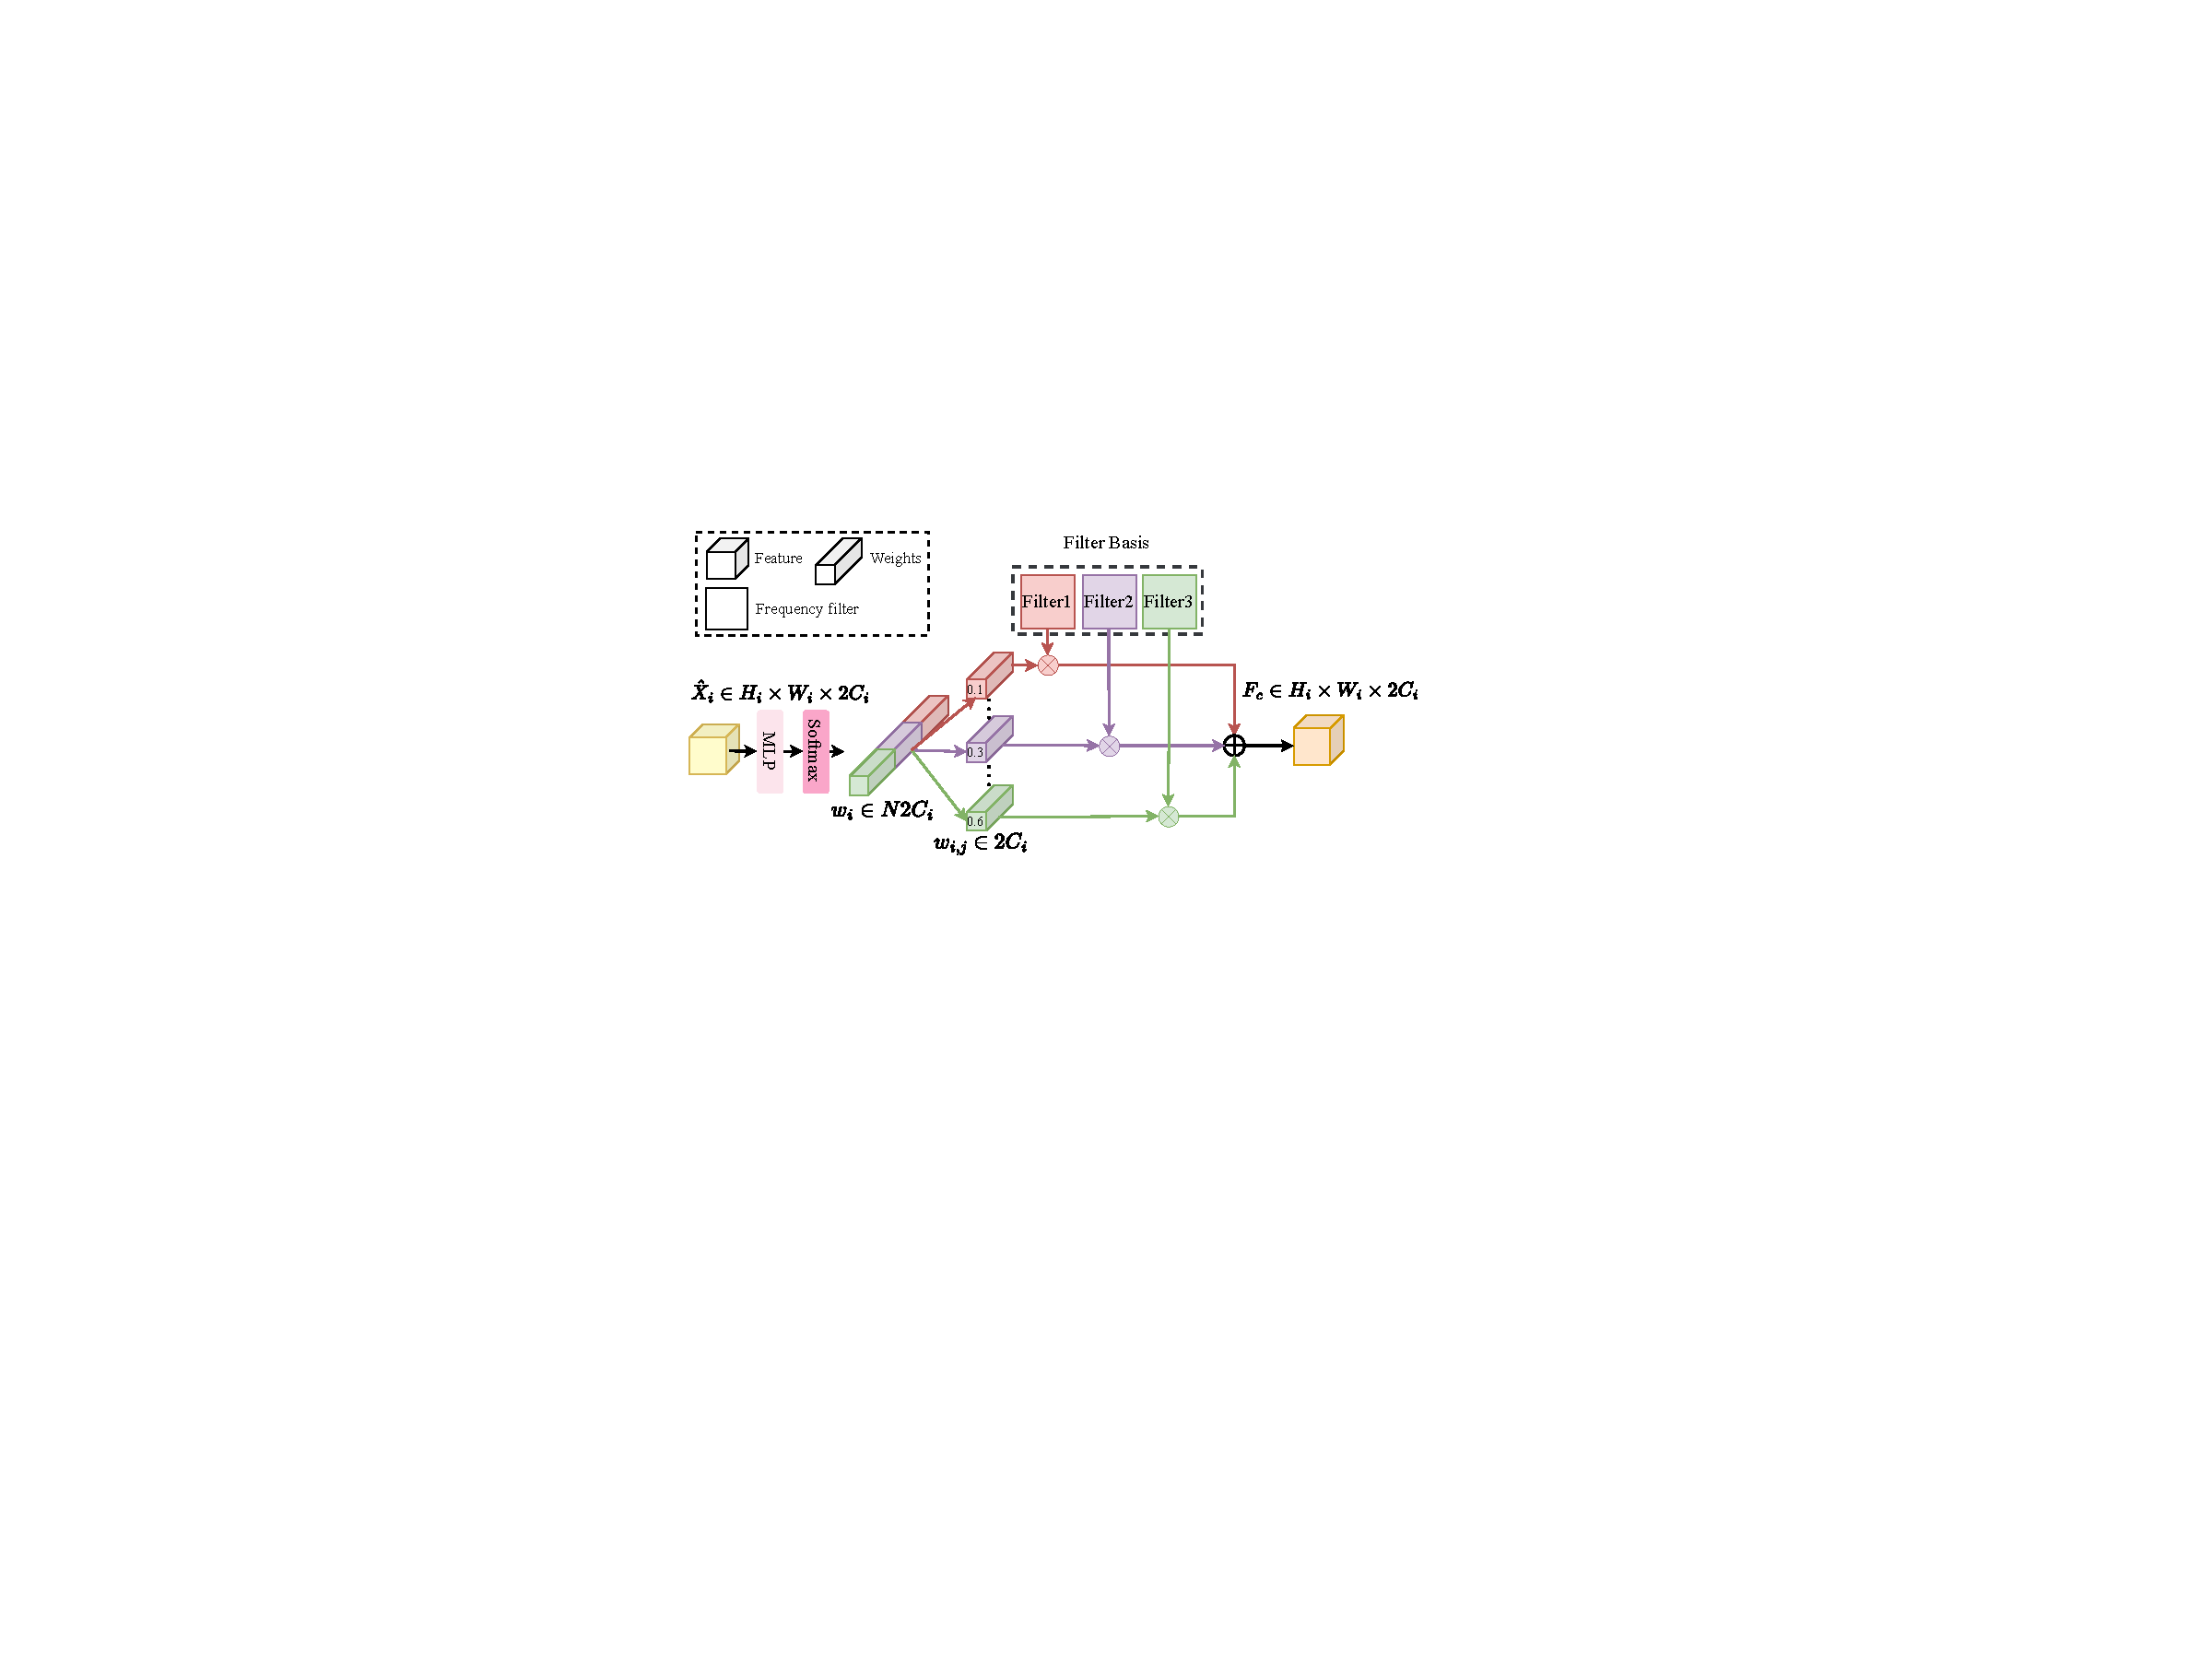
\includegraphics[width=\columnwidth]{AFG.pdf}
\caption{\fontsize{8}{10}\selectfont Illustration of the Adaptive Filter Generator (AF Generator).}
\label{afg}
\end{figure}

\textbf{Adaptive Filter Generator:}
To generate adaptive filters, an MLP followed by softmax normalization produces channel-wise weights that linearly combine a filter basis $\mathbb{M}={\mathcal{M}_1,\ldots,\mathcal{M}_N}$, where each $\mathcal{M}_i\in\mathbb{C}^{H\times\lceil\frac W2\rceil}$ is a randomly initialized complex parameter. Since each spectral channel captures distinct frequency responses, channel-wise filtering is applied, as shown in Fig.~\ref{afg}. The weights are computed as:
\begin{equation}
\mathbf{a}=\text{Softmax}\left(\text{MLP}\left(\frac{\sum_{h=1}^{\text{H}}\sum_{w=1}^{\text{W}} \mathbf{X}_{:,h,w}}{{\text{H}}{\text{W}}}\right)\right),
\end{equation}
\begin{equation}
\mathbf{a}=(\alpha_1,\ldots,\alpha_{N2C})^{\top},
\end{equation}
where $\mathbf{a}\in \mathbb{R}^{N2C}$ weights the filter basis to generate adaptive filters:
\begin{equation}
 \mathbf{F}_c = \sum_{i=1}^{N} \left( \frac{e^{\alpha_{c,i}}}{\sum_{n=1}^{N} e^{\alpha_{c,n}}} \right) \mathcal{M}_i
\end{equation}
where $\alpha{c,i}$ is the $i$-th element of $\alpha$ for the $c$-th group. The vector $\alpha$ is divided into $N$ segments of length $2C$. In our model, we set $N=3$, matching the dimension of $\mathbb{M}$. A larger $N$ increases computational cost, while a smaller $N$ (e.g., $N=1$) degenerates filters into fixed ones.



%第四部分：实验
\section{Experiments}
\subsection{Dataset}
Experiments were conducted on the ACDC~\cite{DeepLearningTechniques2018} and M\&Ms~\cite{MulticentreMultivendorMultidisease2021} datasets following  \cite{MambaUNetUNetPureVisual2024} and \cite{UTNetHybridTransformer2021}, respectively. The ACDC dataset contains 200 annotated cardiac MRI scans from 100 patients, with labels for the right ventricle (RV), myocardium (MYO), and left ventricle (LV). Data are split into 70 training (1{,}930 slices), 10 validation, and 20 testing cases.
The M\&Ms dataset includes 375 patients and 7334 annotated slices from four MRI vendors: A) Siemens, B) Philips, C) GE, and D) Canon. The training set comprises 150 annotated scans, while 25 unannotated scans from vendor~C are excluded. The test set contains 200 cases (50 from each vendor).



\subsection{Implementation Details}
We conduct experiments on a single 16GB NVIDIA RTX~3090 GPU. The input images are resized to $224 \times 224$ and $256 \times 256$ for ACDC and M\&Ms, respectively. The number of training iterations is 15{,}000 for ACDC and 10{,}000 for M\&Ms, with a batch size of 16. Training uses PyTorch 2.1.1 with SGD (lr=0.01, momentum=0.9) and combines cross-entropy and Dice losses, and evaluation employs DSC and \mbox{HD95 metrics.}



\begin{table}[t]
\caption{Comparative experimental results of ACDC dataset.}
\label{acdc results}
\begin{center}
\setlength{\tabcolsep}{5pt} % 列间距
\renewcommand{\arraystretch}{1.1} % 行间距
\begin{tabular}{cccccc}
\hline
\multirow{2}{*}{Methods} & \multicolumn{4}{c}{DSC(\%)$\uparrow$}                                       & \multirow{2}{*}{HD95 (mm)$\downarrow$} \\
                         & RV             & MYO& LV             & Avg            &                            \\ \hline
U-Net\cite{ronnebergerUNetConvolutionalNetworks2015}                     & 85.01          & 86.35          & 94.29          & 88.55          & 2.39                       \\
Swin-Unet\cite{SwinUnetUnetlikePure2021a}                & 85.62          & 84.49          & 94.03          & 88.05          & 2.08                       \\
TransUNet\cite{TransUNetTransformersMake2021}                 & 86.87          & 84.22          & 94.12          & 88.40          & 1.65                       \\ \hline
HiFormer\cite{HiFormerHierarchicalMultiscale2023}                 & 90.51          & 89.27          & 95.68& 91.82& 1.12                       \\
TransCASCADE\cite{MedicalImageSegmentation2023}             & 89.07          & 88.90          & 94.45          & 90.81          & 1.29                       \\
PVT-CASCADE\cite{MedicalImageSegmentation2023}              & 90.15          & \textbf{89.97} & 95.05          & 91.72          & 1.16                       \\ \hline
Swin-UMamba\cite{SwinUMambaMambabasedUNet2024}& 85.12          & 83.73          & 93.81          & 87.55          & 2.47                       \\
UU-mamba\cite{UUmambaUncertaintyawareUmamba2024}                 & 90.23          & 89.43          & 95.60          & 91.75          & 1.20                       \\
Mamba-UNet\cite{MambaUNetUNetPureVisual2024}               & 90.25          & 88.39          & 94.27          & 90.97          & 1.81\\ \hline
\textbf{SAF-Mamba(ours)}    & \textbf{90.87} & 89.42          & \textbf{96.34} & \textbf{92.21} & \textbf{1.05}              \\ \hline
\end{tabular}
\end{center}
\end{table}

 

\begin{table}[t]
\caption{Comparative experimental results of M\&Ms dataset.}
\label{mms results}
\begin{center}
\setlength{\tabcolsep}{4pt} % 缩小列间距
\renewcommand{\arraystretch}{1.1}
\begin{tabular}{ccccccc}
\hline
\multirow{2}{*}{Methods}                                             & \multicolumn{5}{c}{DSC(\%)$\uparrow$}                                              & \multirow{2}{*}{HD95 (mm)$\downarrow$} \\
                                                                     & A              & B              & C              & D              & Avg            &                                        \\ \hline
U-Net\cite{ronnebergerUNetConvolutionalNetworks2015} & 87.65          & 84.80          & 82.69          & 83.79          & 84.73          & 15.85                                  \\
Swin-Unet\cite{SwinUnetUnetlikePure2021a}           & 86.27          & 84.52          & 83.11          & 84.95          & 84.71          & 13.66                                  \\
TransUNet\cite{TransUNetTransformersMake2021}       & 87.69          & 85.82          & 84.25          & 85.53          & 85.82          & 13.30                                  \\ \hline
HiFormer\cite{HiFormerHierarchicalMultiscale2023}   & 87.90          & 83.94          & 83.25          & 83.86          & 84.74          & 12.78                                  \\
TransCASCADE\cite{MedicalImageSegmentation2023}     & 85.92          & 84.23          & 82.93          & 84.43          & 84.38          & 13.91                                  \\
PVT-CASCADE\cite{MedicalImageSegmentation2023}      & 88.71          & 87.12          & 85.36          & 87.81          & 87.25          & 12.60                                  \\ \hline
Swin-UMamba\cite{SwinUMambaMambabasedUNet2024}      & 87.88          & 86.15          & 83.67          & 85.28          & 85.75          & 13.29                                  \\
UU-mamba\cite{UUmambaUncertaintyawareUmamba2024}    & 88.15          & 86.90          & 85.22          & 86.79          & 86.77          & 13.09                                  \\
Mamba-UNet\cite{MambaUNetUNetPureVisual2024}        & 88.32          & 86.48          & 83.11          & 86.98          & 86.22          & 14.05                                  \\ \hline
\textbf{SAF-Mamba(ours)}                                              & \textbf{89.16} & \textbf{88.79} & \textbf{86.83} & \textbf{88.92} & \textbf{88.43} & \textbf{12.14}                         \\ \hline
\end{tabular}
\end{center}
\end{table}

\begin{figure}[t]
\centering
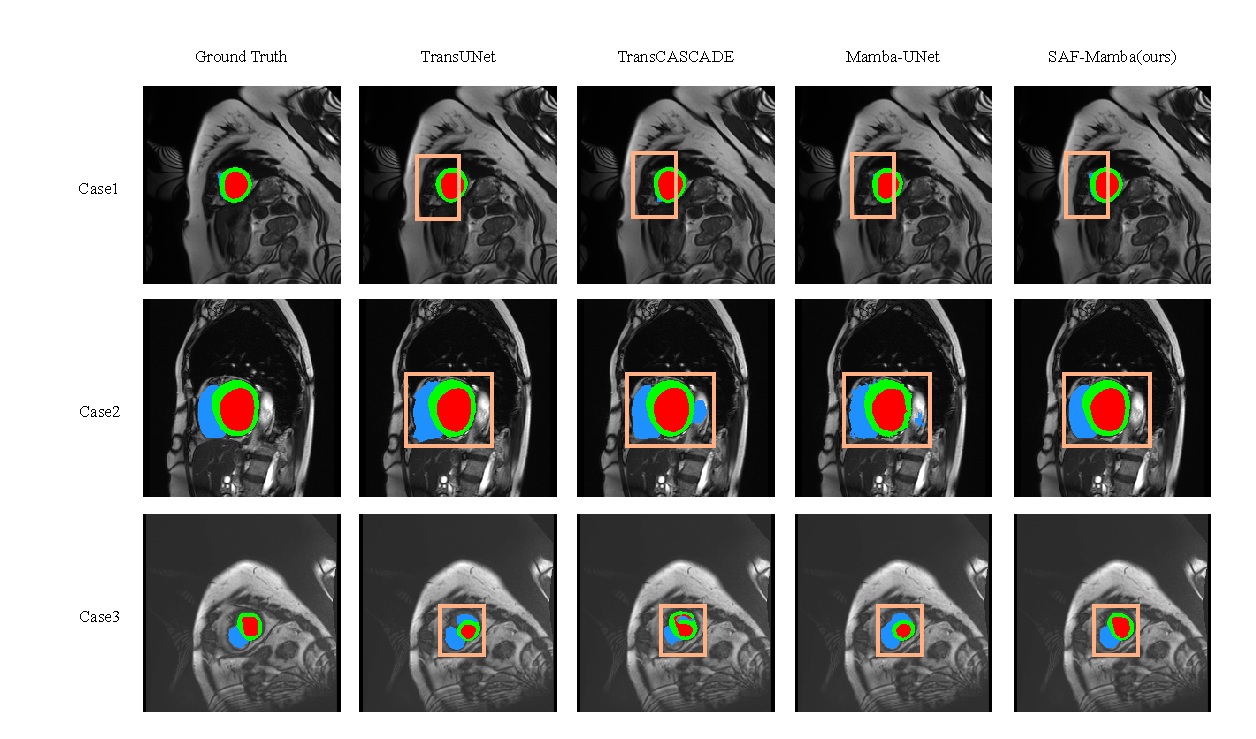
\includegraphics[width=\columnwidth]{segvisual.pdf}
\caption{\fontsize{8}{10}\selectfont The visualization of segmentation results on the ACDC dataset.}
\label{seg}
\end{figure}


\begin{figure}[t]
\centering

\includegraphics[width=\columnwidth]{filters.pdf}
\caption{\fontsize{8}{10}\selectfont The adaptive filter bases in AFBs learned from (a) the ACDC dataset and (b) the M\&M dataset.}
\label{afb}
\end{figure}




\subsection{Comparison Experiments}
\noindent \textbf{Comparison with State-of-the-arts:}
We compare SAF-Mamba with nine state-of-the-art (SOTA) methods, including CNN-, Transformer-, and Mamba-based approaches. 
As shown in Table~\ref{acdc results}, SAF-Mamba achieves the highest average DSC (92.21\%) and the lowest HD95 (1.05~mm) on the ACDC dataset, particularly improving RV segmentation and boundary accuracy. 
On the M\&Ms dataset (Table~\ref{mms results}), it also attains the best mean DSC (88.43\%) and HD95 (12.14), demonstrating strong robustness and cross-vendor generalization.

\noindent \textbf{Visual Comparison:}
Qualitative examples in Fig.~\ref{seg} show that SAF-Mamba produces smoother and more accurate contours than other methods, especially in low-contrast or irregular regions.

\noindent \textbf{Visualization of Adaptive Filter Basis:}
Fig.~\ref{afb} illustrates that the learned filters exhibit diverse high-, low-, and band-pass patterns across stages, validating the adaptive frequency modulation capability of AFB.

\begin{table}[H]
\caption{The results of ablation studies conducted on ACDC dataset.}
\label{ablation}
\begin{center}
\renewcommand{\arraystretch}{1.1} % 行间距
\begin{tabular}{ccccc}
\hline
Methods                    & MSVSS & AFB & DSC(\%)$\uparrow$  & HD95(mm)$\downarrow$ \\ \hline
\multirow{4}{*}{\centering SAF-Mamba(ours)}                 & \ding{55} & \ding{55} & 90.97 & 1.81 \\
                           & \checkmark  & \ding{55} & 91.25 & 1.47 \\
                           & \ding{55} & \checkmark  & 91.54 & 1.42 \\
                           & \checkmark  & \checkmark  & 92.21 & 1.05 \\\hline
\end{tabular}
\end{center}
\end{table}


\subsection{Ablation Studies}
We conduct ablation experiments on the ACDC dataset to evaluate each module’s contribution. Removing either MSVSS or AFB reduces accuracy, indicating their complementary roles. When both modules are integrated, SAF-Mamba achieves the highest DSC of 92.21\% and HD95 of 1.05 mm, validating their joint effectiveness.





\section{Conclusion}
In this paper, we propose SAF-Mamba, a novel cardiac image segmentation method addressing two main challenges: scale variation and boundary displacement. The proposed dual-branch architecture effectively captures multi-scale information, while adaptive filtering enhances frequency-domain details. Experiments on the two public datasets demonstrate that our method enables  more efficient and accurate computer-aided diagnosis, particularly in cardiovascular disease detection and intervention.





\bibliographystyle{IEEEtran}
\bibliography{bibm2025references,IEEEtranBSTControl}


\end{document}